%XeLaTeX
\documentclass[14pt, oneside]{altsu-report}

\worktype{Отчёт по технологической (проектно-технологической) практике на тему:}
\title{РАЗРАБОТКА КРОССПЛАТФОРМЕННОГО ИГРОВОГО ПРИЛОЖЕНИЯ FLAPPY BIRD ДЛЯ LINUX и WINDOWS С ГРАФИЧЕСКИМ ИНТЕРФЕЙСОМ}
\author{В.\,Г.~Иванова}
\groupnumber{5.205-1}
\GradebookNumber{1337}
\supervisor{И.\,А.~Шмаков}
\supervisordegree{ст.пр. кафедры ВТиЭ}
\ministry{Министерство науки и высшего образования}
\country{Российской Федерации}
\fulluniversityname{ФГБОУ ВО Алтайский государственный университет}
\institute{Институт цифровых технологий, электроники и физики}
\department{Кафедра вычислительной техники и электроники}
\departmentchief{В.\,В.~Пашнев}
\departmentchiefdegree{к.ф.-м.н., доцент}
\shortdepartment{ВТиЭ}
\abstractRU{Данная работа посвящена разработке кроссплатформенного игрового приложения в Unity. Целью является создание игры «Flappy Bird» с графическим интерфейсом для таких операционных систем как Linux и Windows на языке C\#. Для выполнения поставленной задачи необходимо было изучить литературу по данной теме. 
}

\abstractEN{This work is devoted to the development of a cross-platform game application in Unity. The goal is to create a "Flappy Bird" game with a graphical interface for operating systems such as Linux and Windows in C\#. To complete the task, it was necessary to study the literature on this topic. 
}

%\keysRU{компьютерное моделирование, cистема управления версиями}
%\keysEN{computer simulation, distributed version control}

\date{\the\year}

% Подключение файлов с библиотекой.
\addbibresource{graduate-students.bib}

% Пакет для отладки отступов.
%\usepackage{showframe}

\begin{document}
\maketitle

\setcounter{page}{2}
\makeabstract
\tableofcontents

\chapter*{Введение}
\phantomsection\addcontentsline{toc}{chapter}{ВВЕДЕНИЕ}

Индустрия компьютерных игр является одной из самой перспективной и быстроразвивающейся областью в мире информационных технологий. Игры находят в себе не только развлекательный характер, но и учебный, что способствует развитию различных качеств как у взрослых, так и у детей. Например, игры способны развивать внимание, общительность, формируют логическое мышление, расширяют кругозор. Существуют также разные категории игр, которые делают упор в большую степень развития качеств человека.

На сегодняшний день создание игровых приложений не ограничивает пользователей различных операционных систем, что позволяет разрабатывать игры, которые никак не будут конфликтовать между разными платформами. Благодаря использованию кросс-платформенных инструментов и технологий, разработчики могут создавать игровые приложения, которые могут быть запущены на разных устройствах, таких как персональные компьютеры, смартфоны, планшеты и игровые консоли.

В данной работе будет разработано приложение под  Linux и Windows под известным названием «Flappy Bird» с помощью кроссплатформенной среды Unity.

\textbf{Актуальность:} 
Актуальность данной работы заключается в использовании кросс-платформенных инструментов и технологий для создания игрового приложения, которое может быть запущено на разных устройствах. 

\textbf{Цель:}
Целью данной работы является разработка кроссплатформенного игрового приложения «Flappy Bird» с графическим интерфейсом для таких операционных систем как Linux и Windows.

\textbf{Задачи:}
\begin{enumerate}
\item Изучить кроссплатформенную среду разработки компьютерных игр Unity.
\item Изучить стандартную библиотеку С\#.
\item Изучить использование методов С\# в Unity.
\item Спроектировать игровую механику игры Flappy Bird.
\item Внедрить игровой интерфейс к игре.
\item Выявить и исправить возможные ошибки при разработке игры.
\end{enumerate}

Благодаря данной работе можно будет на практике применять свои навыки программирования на C\# и использование среды Unity в дальнейшем, а также расширить имеющиеся знания и области применения данного языка и платформы, так как это актуально в современном мире.


\chapter{ГЛАВА 1. ТЕОРЕТИЧЕСКАЯ ЧАСТЬ} 

Создание игровых приложений стало более доступным и простым благодаря развитию интегрированных сред разработки (IDE) и готовых игровых движков, которые предоставляют широкий набор инструментов и ресурсов для разработки игр. Это позволяет как профессионалам, так и начинающим разработчикам воплощать свои идеи в жизнь и создавать качественные игровые продукты.

Одной из такие сред и является Unity - кроссплатформенная среда разработки игр ~\cite{Unity18}.  

Кроссплатформенность - это способность программного обеспечения работать с несколькими операционными системами ~\cite{Unity19}. 

Unity предлагает моделирование физических сред, карты нормалей, преграждение окружающего света в экранном пространстве, динамические тени и т.д.  ~\cite{Unity20}. 

У среды также есть основные преимущества перед другими инструментами разработки игр:

\begin{enumerate}
\item Производительный визуальный рабочий процесс.
\item Межплатформенная поддержка.
\end{enumerate} 

Unity поддерживает различные платформы, включая ПК, мобильные устройства, игровые консоли, виртуальную и дополненную реальность ~\cite{Unity, Unity2, Unity5}.

Платформа также предлагает широкий выбор ресурсов, что позволяет разработчикам использовать готовые модели, текстуры и другие элементы для ускорения процесса разработки игры. 

Данная среда использует язык программирования C\# в качестве основного языка разработки. C\# - это объектно-ориентированный язык программирования, разработанный Microsoft. Он предоставляет возможности для разработки игр и приложений, включая синтаксическую ясность, безопасность типов, а также удобные инструменты для управления памятью.

Unity обеспечивает интеграцию с языком C\# и предоставляет разработчикам широкий набор программирования, который позволяет взаимодействовать с различными компонентами и системами игрового движка. Разработчики могут использовать C\# для создания игровой логики, управления объектами и персонажами, работы с анимацией и многого другого. 

C\# в Unity имеет множество преимуществ, включая хорошую производительность, удобство разработки и интеграцию с другими инструментами среды. Платформа также предоставляет среду разработки Visual Studio и Visual Studio Code, которые обеспечивают инструменты для отладки с помощью скриптов ~\cite{Unity3, Unity4}. 

Благодаря своей гибкости и мощным возможностям, Unity стал одним из популярных инструментов для разработки игр и приложений в игровой индустрии.

В данной среде будет разрабатываться приложение под названием «Flappy Bird» — это игра на реакцию. В ней нужно управлять птичкой и пролететь через трубы.

Управление птичкой - для поддержания полета достаточно нажимать на левую кнопку мыши или пробел на клавиатуре. Цель игры — пролететь возможное большее расстояние. Если птичка сталкивается с трубой, то игра завершается. После проигрыша можно начать игру заново ~\cite{Unity10}.

Основной используемый класс в коде MonoBehaviour, когда создается сценарий C\#, он автоматически подключается. Класс позволяет запускать, останавливать и управлять программными модулями ~\cite{Unity6}. 

В MonoBehaviour содержатся такие функции как:

\begin{enumerate}
\item Awake() -- вызывается при запуске сцены или при активации объекта. Метод предоставляет доступ к компоненту, который отвечает за отображение спрайтов на экране, и сохраняет его ссылку, чтобы можно было взаимодействовать с ним в других методах этого скрипта. ~\cite{Unity13}.
\item Start() -- вызывается только один раз для дополнительных операций ~\cite{Unity14}.
\item Update() -- вызывается каждый кадр во время выполнения игры и используется для обновления состояния компонента и выполнения обработки ввода пользователя, обновления позиции объектов, анимации, физики и других изменений, которые должны происходить каждый кадр игры ~\cite{Unity15}.
\item OnTriggerEnter2D(Collider2D other) -- OnTriggerEnter2D(Collider2D other) - вызывается, когда коллайдер данного объекта входит в триггер другого объекта в двухмерном пространстве ~\cite{Unity16}.
\item OnEnable() -- вызывается, когда компонент становится активным, а также при каждой последующей активации после его отключения ~\cite{Unity17}.

\end{enumerate} 

Также в дальнейшем будут встречаться такие термины как скрипт, спрайты и префаб. 

Скрипт — это компонент, который разработчик игр создает самостоятельно для реализации каких-то свойств и возможностей игровых объектов, которые невозможно сделать при помощи встроенных компонентов Юнити. Скриптов у объекта может быть несколько и каждый из них может выполнять разные задачи~\cite{Unity8}. 

Спрайты - картинки в 2D-играх, из которых состоят игровые персонажи, движущиеся объекты и т.д~\cite{Unity9}. 

Префаб - это шаблон для объекта в Unity. С их помощью можно создать «образец» предмета с определенными свойствами, а потом использовать такие предметы на всей игровой сцене. Если изменить префаб, то изменятся все объекты, созданные на его основе. Это структурирует и оптимизирует процесс, а также создает четку и понятную иерархию объектов ~\cite{Unity7}.


\chapter{ГЛАВА 2. ПРАКТИЧЕСКАЯ ЧАСТЬ}

\textbf{Подготовка к разработке}

Разработка игры начинается с создания проекта в среде Unity. Он будет называться «Flappy2D». Вся разработка приложения будет идти на версии 2021.3.4f1. Далее выбирается 2D шаблон разработки, так как сама игра «Flappy Bird» разработана под двухмерное пространство. 

Данный шаблон заранее включает различные 2D-пакеты для разработки таких игр. 

Например это: 

\begin{enumerate}
\item 2D-анимация.
\item Двумерные источники света.
\item Sprite Shape (создание окружения с помощью различных форм).
\item Tilemaps (создание шестиугольные и изометрические карты)~\cite{Unity11}.
\end{enumerate}  

При создании игры понадобятся 2D-анимации и  Sprite Shape. Самое важное, что этот пакет разработан под платформы iOS, Android, Linux, macOS, WebGL, Windows, а значит он обладает нужной кроссплатформенностью под цели работы.

При загрузке рабочего пространства Unity выдаст нам что-то по типу «сцены», в которой и начнется разработка. Для начала добавим спрайты в папку «Kartinks», к части которых будут писаться в дальнейшем скрипты, проектироваться анимация и разрабатываться окружение с помощью различных фигур.

В данном проекте будет 19 спрайтов:

\begin{enumerate}
\item Bird01, Bird02, Bird03 - спрайты для птички. Из них будет создаваться анимация полета.
\item Background - задний фон, над которым можно будет поработать с помощью пакета Sprite Shape.
\item Pipe - трубы.
\item Ground - земля локации из которой будут исходить трубы.
\item About и AboutImage - первый спрайт будет служить кнопкой в игре для открытия информации о разработчике, второй служит той самой информацией.
\item Exit - служит кнопкой в игре для выхода из нее.
\item FlappyBird - спрайт с названием игры для главного экрана.
\item GameOver - появляется после окончания попытки игры, что дает понять, что игра завершена.
\item Help и H - первый спрайт будет служить кнопкой в игре для открытия информации об игре, второй служит той самой информацией.
\item Panel - спрайт для вставки рекордов, чтобы в игре это органично смотрелось.
\item Pause и Start - служат кнопками в игре. Первая останавливает игру, чтобы поставить ее на паузу, вторая наоборот возобновляет.
\item PlayButton - служит кнопкой старта игры и ее дальнейшего перезапуска.
\item StartOcho2 и RecordOcho2 - спрайт с информацией об видах очков. Первый определяет сколько очков за игру было набрано, второй - максимальный рекорд за сеанс.
\end{enumerate} 

После добавления спрайтов им можно изменить настройки импорта, что и сделается для всех картинок для более правильной композиции игры ~\cite{Unity12}.

По умолчанию Pixels Per Unit = 100. 100 пикселей на единицу будет означать, что спрайт, который равен 100 пикселям, будет равен 1 единице сцены. Это расширение слишком большое для проекта. Например, та же самая птичка на сцене будет очень маленькой. Оптимальнее будет поставить Pixels Per Unit = 24.

Format = RGBA 32 bit. Ставится для того, чтобы не было резкого перехода цветов.

Max Size = 256. Ставится из-за того, что размеры спрайтов не превышают данное значение.

Filter Mode = Point(no filter). Когда установлено значение «Point», текстуры не подвергаются фильтрации при масштабировании, что означает, что каждый пиксель исходной текстуры будет соответствовать одному пикселю на экране. Это используется для сохранения пиксельности этой игры.

После данных действий можно начать добавлять на сцену элементы игры и писать к ним скрипты.

\textbf{Программирование птички}

После добавления птички на сцену, ей нужно задать дополнительные компоненты. В разделе «Tag» мы выбираем «Player», это делается для того, чтобы создать некое единство игры с главным объектом, на который в последствии можно будет ссылаться. То есть, объекту птички мы просто присваиваем метку или идентификатор.

Добавим дополнительно компонент Rigidbody 2D. Он в Unity является компонентом, который используется для моделирования физики движения 2D объектов. Коомпонент применяется к игровому объекту и позволяет симулировать движение, столкновения и взаимодействия сил в двумерной сцене. Здесь птичке нужно задать Bode Type = Kinematic. Когда установлено это значение, объекты с таким компонентом игнорируют физическую симуляцию и не подвергаются воздействию сил гравитации, столкновений или других физических эффектов.

Также добавим Circle Collaider 2D. Это компонент в Unity, который используется для определения области в форме круга для 2D объектов, то есть он используется для обнаружения столкновений с другими объектами и взаимодействия с ними на основе формы круга. Так как птичка имеет приближенную форму круга, ей данный компонент будет подходить, единственное, нужно изменить радиус под ее формы. Таким образом Radius = 0,23.

Теперь можно начать писать скрипт под названием «Player» для этого объекта. Все скрипты будут храниться в папке «Scripts». Для того, чтобы этот сценарий работал, его надо перетащить ко всем компонентам объекту птички, только тогда он станет единым целым с птичкой. 

Данный скрипт реализует прыжки птички с гравитацией, анимацию ее спрайтов, обработку пользовательского ввода для управления объектом и ее столкновение с трубами, счет очков через них и обнуление позиции птички, чтобы она начинала каждую игру с центра, а не с того места, где упала.

В коде используются функции:

\begin{enumerate}
\item Awake() - вызывается при запуске сцены или при активации объекта. Метод предоставляет доступ к компоненту, который отвечает за отображение спрайтов на экране, и сохраняет его ссылку, чтобы можно было взаимодействовать с ним в других методах этого скрипта.
\item Start() - вызывается один раз при запуске сцены. Используется для анимации, каждые 0.15 секунд спрайты меняются по порядку.
\item Update() - вызывается каждый кадр и используется для обработки ввода пользователя и обновления состояния игрового объекта. В коде проверяется нажатие клавиши пробела или левой кнопки мыши. Если нажатие произошло, устанавливается направление прыжка птички вверх с заданной силой. Затем к направлению добавляется влияние гравитации, чтобы птичка падала. После этого обновляется позиция объекта.
\item AnimateSprite() - метод, отвечающий за анимацию спрайтов птички. Увеличивает значение индекса спрайтов для переключения на следующий спрайт из массива спрайтов. Если индекс превышает или равен длине массива, то возвращается к началу анимации. Затем устанавливается текущий спрайт для отображения на экране.
\item OnEnable() - вызывается при включении компонента. Она центрирует птичку по вертикали, устанавливая ее позицию y на 0. Также переменная direction устанавливается в нулевой вектор.
\item OnTriggerEnter2D(Collider2D other) - вызывается, когда птичка сталкивается с другим объектом в 2D-пространстве. В коде проверяется тег объекта столкновения. Если тег равен "Barrier", то вызывается функция GameOver() компонента GameManager, что приводит к завершению игры. Если тег равен "Ochos", то вызывается функция IncreaseScore() компонента GameManager, что увеличивает счет очков игры.
\end{enumerate} 

Написанный скрипт подробно расписан в приложении под заголовком «Код для объекта Player (Птички)».

\begin{figure}[H]
\center{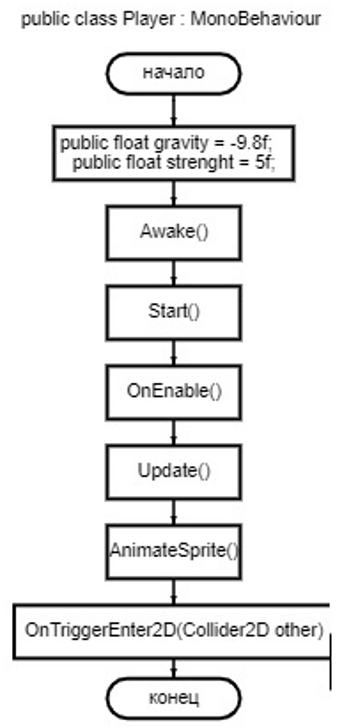
\includegraphics[scale=1.2]{p/PlayerOsn.png}}
\caption{Блок-схема для класса Player.}
\end{figure}

Блок-схемы для функций в классе Player:
\begin{enumerate}
\item Awake() 

\begin{figure}[H]
\center{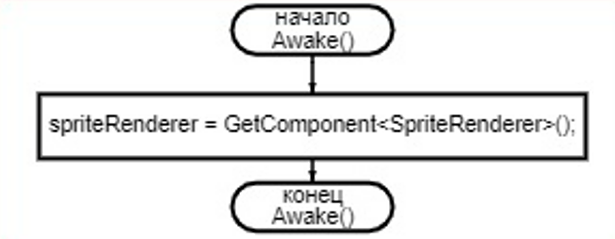
\includegraphics[scale=1.2]{p/PlayerOsnAwake.png}}
\caption{Блок-схема для функции Awake() в классе Player.}
\end{figure}

\item Start() 

\begin{figure}[H]
\center{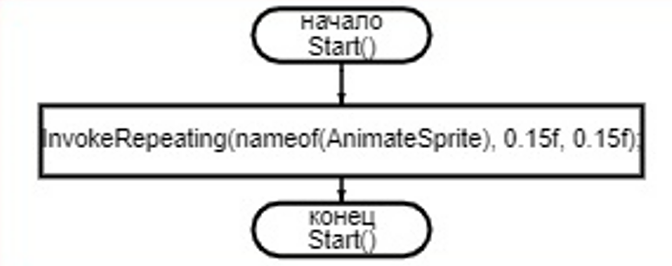
\includegraphics[scale=1.2]{p/PlayerOsnStart.png}}
\caption{Блок-схема для функции Start() в классе Player.}
\end{figure}

\item Update() 

\begin{figure}[H]
\center{\includegraphics[scale=0.8]{p/PlayerOsnUpdate.png}}
\caption{Блок-схема для функции Update()  в классе Player.}
\end{figure}


\item AnimateSprite()

\begin{figure}[H]
\center{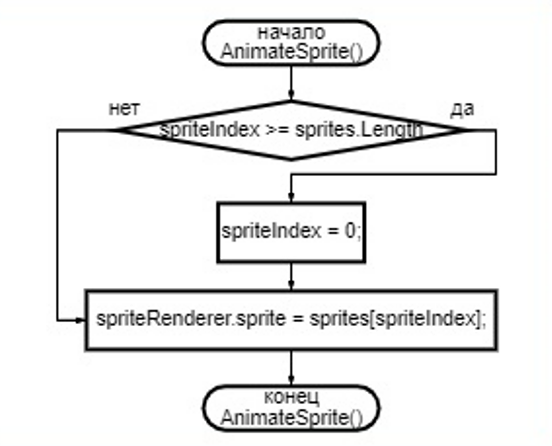
\includegraphics[scale=1.2]{p/PlayerOsnAnimateSprite.png}}
\caption{Блок-схема для функции AnimateSprite() в классе Player.}
\end{figure}


\item OnEnable() 

\begin{figure}[H]
\center{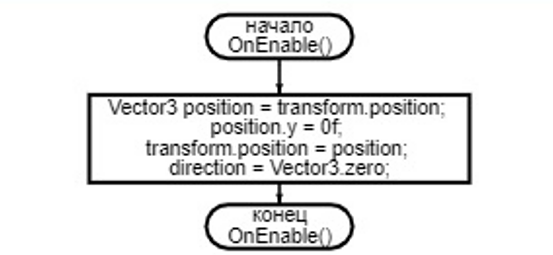
\includegraphics[scale=1.2]{p/PlayerOsnAnimateOnEnable.png}}
\caption{Блок-схема для функции OnEnable() в классе Player.}
\end{figure}


\item OnTriggerEnter2D(Collider2D other) 

\begin{figure}[H]
\center{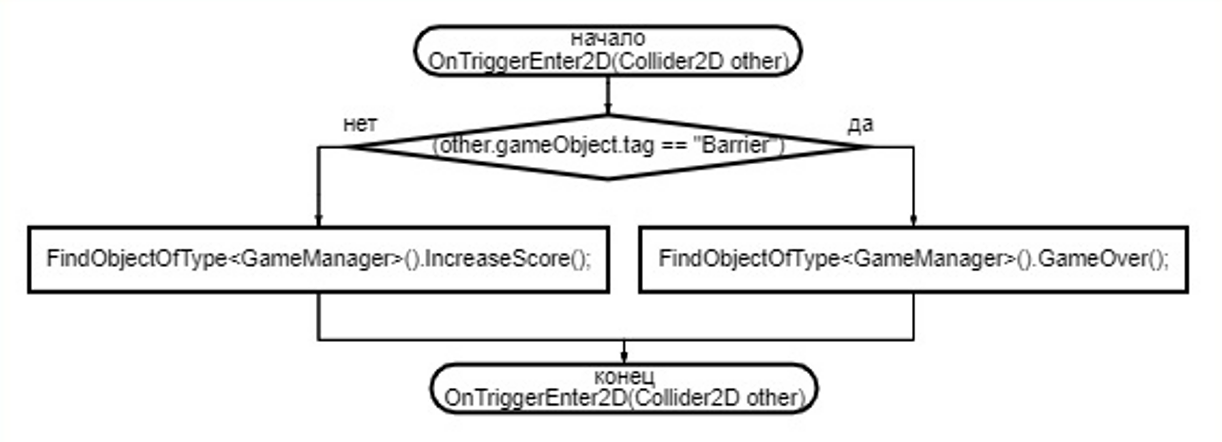
\includegraphics[scale=0.68]{p/PlayerOsnAnimateOnTriggerEnter2D.png}}
\caption{Блок-схема для функции OnTriggerEnter2D(Collider2D other) в классе Player.}
\end{figure}


\end{enumerate}

\textbf{Подготовка и программирование заднего фона}

Перед созданием фона нужно отредактировать параметры спрайта Background, поставив в Wrap Mode = Repeat. Данная настройка позволяет повторять текстуру по горизонтали и вертикали вместо того, чтобы отображать ее только один раз. Это пригодится при дальнейшем проектировании.

Далее создадим 3D-объект Quad под названием «Back», после этого поместим в папку Back материал под названием Fon. В настройках необходимо выбрать параметры Unlit/Texture и поместить в контроллер спрайт с фоном. Данная настройка будет отображать только текстуру без учета освещения или отражений, в игре это не понадобится. 

На сцене появляется маленький квадрат с фоном, который нужно отредактировать. Сначала его можно просто растянуть, поменяв параметры Scale по x = 25 и y = 15. Чтобы сделать фон более привлекательным, его можно разбить на плитку. В разделе с материалом поставить в Tiling x = 3, этот параметр отобразит одно изображение три раза.  

Теперь можно начать писать скрипт под названием «Back» для этого объекта. Данный скрипт реализует бесконечную прокрутку карты. 

В коде используются методы:

\begin{enumerate}
\item Awake() - вызывается при запуске сцены или при активации объекта. Метод предоставляет доступ к компоненту MeshRenderer, который отвечает за отображение спрайтов на экране, и сохраняет ссылку, чтобы можно было взаимодействовать с ним в других методах этого скрипта.
\item Update() - вызывается каждый кадр и используется для обработки ввода пользователя и обновления состояния игрового объекта. В коде внутри метода происходит обновление смещения главной текстуры (фона/материала) на компоненте MeshRenderer.
\end{enumerate} 

Написанный скрипт подробно расписан в приложении под заголовком «Код для объекта Back (Задний фон)».

\begin{figure}[H]
\center{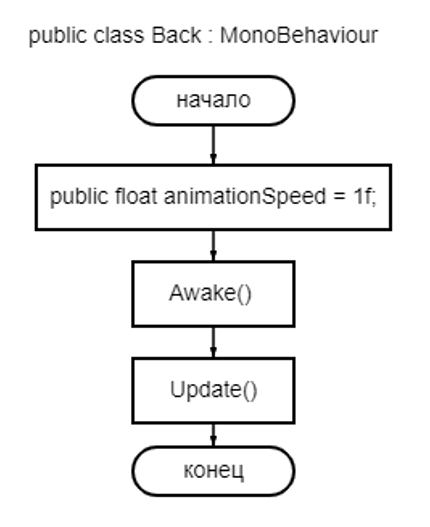
\includegraphics[scale=1.2]{p/BackOsn.png}}
\caption{Блок-схема для класса Back.}
\end{figure}

Блок-схемы для функций в классе Back:
\begin{enumerate}
\item Awake() 

\begin{figure}[H]
\center{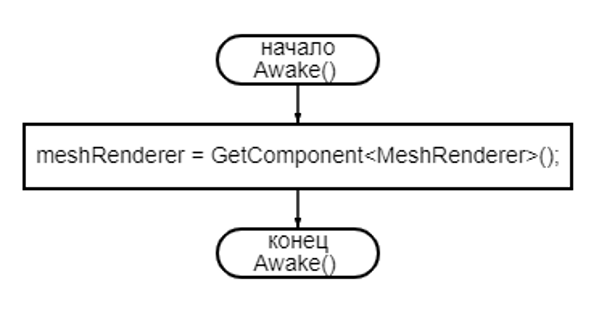
\includegraphics[scale=1.2]{p/BackOsnAwake.png}}
\caption{Блок-схема для функции Awake() в классе Back.}
\end{figure}

\item Update()

\begin{figure}[H]
\center{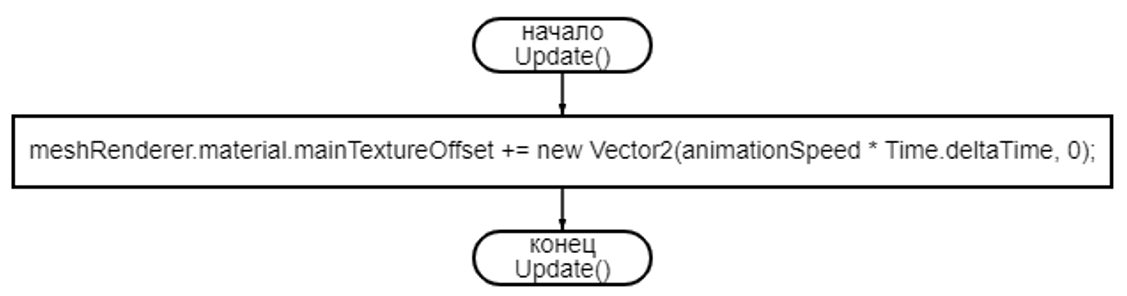
\includegraphics[scale=0.75]{p/BackOsnUpdate.png}}
\caption{Блок-схема для функции Update() в классе Back.}
\end{figure}

\end{enumerate}

\textbf{Подготовка и программирование переднего фона}

Перед созданием фона нужно отредактировать параметры спрайта Ground, поставив в Wrap Mode = Repeat. Данная настройка позволяет повторять текстуру по горизонтали и вертикали вместо того, чтобы отображать ее только один раз. Дополнительно нужен компонент Box Collider 2D, где нужно поставить галочку напротив Is Trigger, что не даст птичке вылетать за карту. Это пригодится при дальнейшем проектировании.

Далее создадим 3D-объект Quad под названием «Ground», после этого поместим в папку Back материал под названием Fon2. В настройках необходимо выбрать параметры Unlit/Texture и поместить в контроллер спрайт с фоном. Данная настройка будет отображать только текстуру без учета освещения или отражений, в игре это не понадобится. 

На сцене появляется маленький квадрат с фоном, который нужно отредактировать. Сначала его можно просто растянуть, поменяв параметры Scale по x = 25 и y = 3, Position по z = -1 для того, чтобы поместить спрайт поверх заднего фона и y = -5.5, чтобы земля находилась внизу. 

Чтобы сделать фон более привлекательным, его можно разбить на плитку. В разделе с материалом поставить Tiling = 3, этот параметр отобразит одно изображение три раза.  

Для переднего фона можно оставить скрипт с заднего фона, изменив лишь скорость прокрутки объекта на animationSpeed = 0.75, чтобы создать эффект разного движения фонов. Он подробно расписан в приложении под заголовком «Код для объекта Ground (Задний фон)».

\begin{figure}[H]
\center{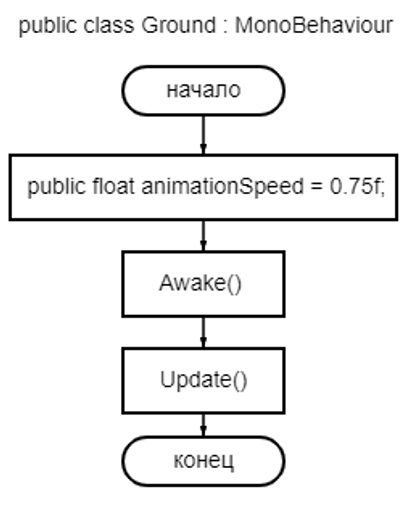
\includegraphics[scale=1.2]{p/GroundOsn.png}}
\caption{Блок-схема для класса Ground.}
\end{figure}

Блок-схемы для функций в классе Back:
\begin{enumerate}
\item Awake() 

\begin{figure}[H]
\center{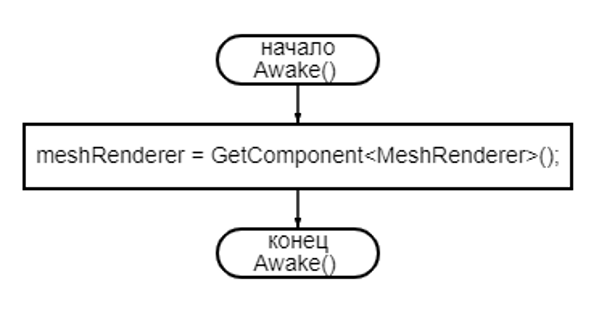
\includegraphics[scale=1.2]{p/GroundOsnAwake.png}}
\caption{Блок-схема для функции Awake() в классе Ground.}
\end{figure}

\item Update()
\begin{figure}[H]
\center{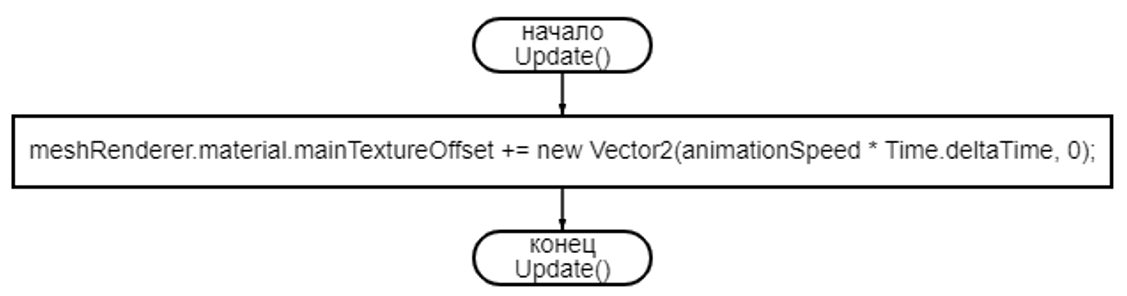
\includegraphics[scale=0.75]{p/GroundOsnUpdate.png}}
\caption{Блок-схема для функции Update() в классе Ground.}
\end{figure}

\end{enumerate}

\textbf{Подготовка и программирование труб}

Здесь уже нужно воспользоваться префабами. Создается основной объект Pipes и в него включаются дополнительно объекты Pipe1, Pipe2, Ocho. В каждом из них создается компонент Box Collaider 2D - он используется для задания простой прямоугольной области столкновения для 2D объектов. Дополнительно у каждого объекта свои параметры: 

\begin{enumerate}
\item Pipe1 - верхняя труба с параметрами Position y = 5.5 и Rotation x = 180. Box Collaider 2D = Is Trigger.
\item Pipe2 - нижняя труба с параметрами  y = -4.5. Box Collaider 2D = Is Trigger.
\item Ocho - в компоненте Box Collider 2D проставляется галочка напротив свойства Is Trigger. Благодаря данной настройке можно установить зону, в которой будет проходить столкновение. Парамеры этой зоны Offset x = 0, y = 0.5 и Size x = 0.4, y = 4.
\end{enumerate} 

Из данных элементов формируется в папке Prefabs префаб под названием «Pipes»

Также создается объект «Prefabs» и устанавливается Position = 10.

Теперь можно начать писать скрипт под названием «Pipe» для этого префаба, который будет спавнить трубы в определенном диапазоне. Этот диапазон увеличивается со смещением во времени, чтобы усложнить игру. В скрипт также добавляется изготовленный префаб. 

В коде используются методы:

\begin{enumerate}
\item OnEnable() - используется для вызова метода Spawn() с определенной частотой, используя InvokeRepeating(). Таким образом, каждую секунду будет создаваться новая труба.
\item Spawn() - создает новую трубу на основе префаба. Он генерирует случайную высоту в заданном диапазоне startminHeight - startmaxHeight и устанавливает позицию созданной трубы с учетом этой случайной высоты. Затем метод использует Instantiate() для создания новой трубы на основе префаба.
\item ResetStartHeight() - пользовательский метод, который сбрасывает начальную высоту спавна труб, устанавливая значения startminHeight и startmaxHeight равной 0.0f. Если говорить наперед, то созданная в дальнейшем кнопка Button для начала игры как раз таки и будет иметь возможность сбрасывать параметры startminHeight и startmaxHeight, чтобы заново установить высоту труб 0.0f.
\end{enumerate} 

Скрипт подробно расписан в приложении под заголовком «Код для объекта Prefabs (Спавн труб)».

\begin{figure}[H]
\center{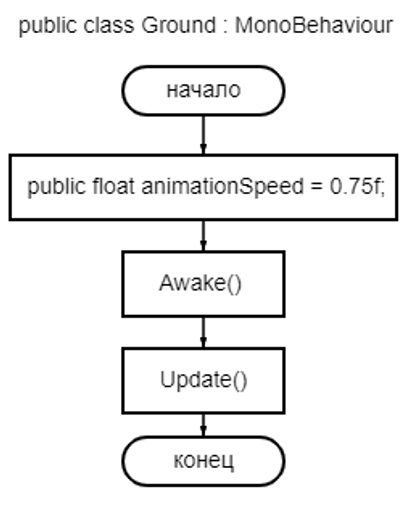
\includegraphics[scale=1.2]{p/GroundOsn.png}}
\caption{Блок-схема для класса Pipe.}
\end{figure}

Блок-схемы для функций в классе Pipe:
\begin{enumerate}
\item OnEnable()

\begin{figure}[H]
\center{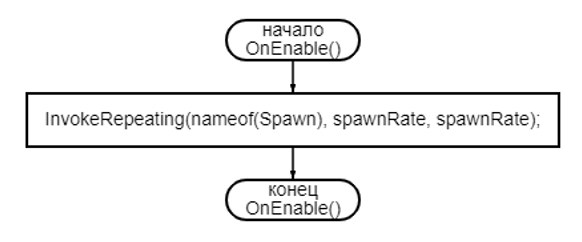
\includegraphics[scale=1.2]{p/PipeOsnOnEnable.png}}
\caption{Блок-схема для функции  OnEnable() в классе Pipe.}
\end{figure}

\item Spawn()

\begin{figure}[H]
\center{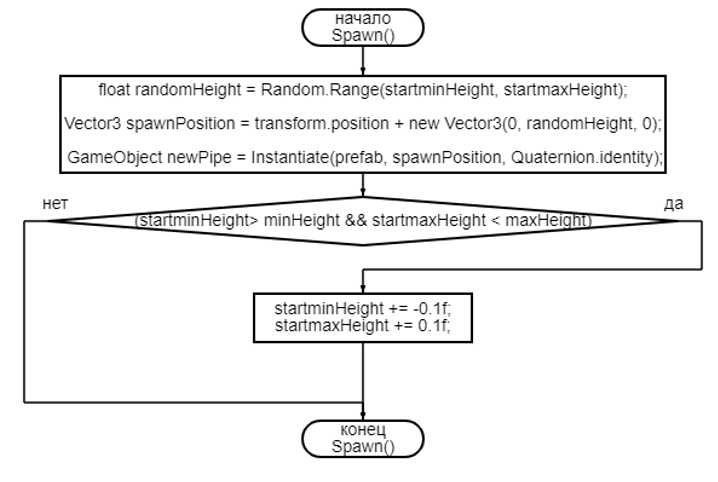
\includegraphics[scale=0.75]{p/PipeOsnSpawn.png}}
\caption{Блок-схема для функции Spawn() в классе Pipe.}
\end{figure}

\item ResetStartHeight()

\begin{figure}[H]
\center{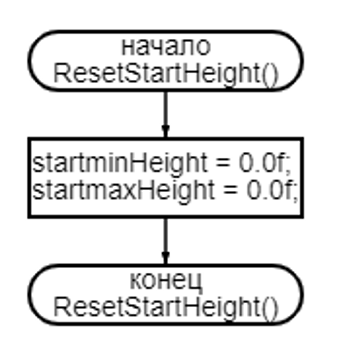
\includegraphics[scale=0.75]{p/PipeOsnReset.png}}
\caption{Блок-схема для функции ResetStartHeight() в классе Pipe.}
\end{figure}

\end{enumerate}

Также для префаба с трубами нужно создать их движение и уничтожение, если они касаются левого края главного экрана. 

В коде используются методы:

\begin{enumerate}
\item Start() - в методе устанавливается значение leftEdge, которое равно координате x левого края главного экрана сцены со сдвигом -1f. Это делается, чтобы трубы исчезали чуть позже, чем когда их центр достигает левого края экрана.
\item Update() - вызывается для перемещения труб влево. Также проверяется, достигла ли труба левого края экрана. Если это условие выполняется, то объект трубы уничтожается.
\end{enumerate} 

Скрипт под названием «PipesD» подробно расписан в приложении под заголовком «Код для префаба Pipes (Движение труб)».

\begin{figure}[H]
\center{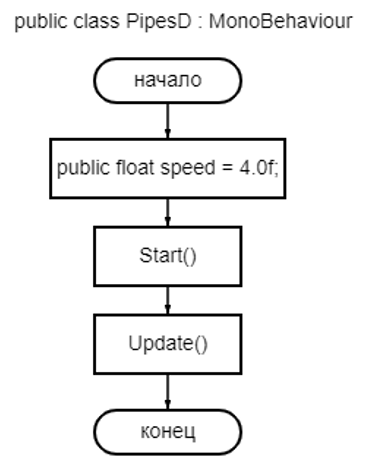
\includegraphics[scale=1.2]{p/PipeDOsn.png}}
\caption{Блок-схема для класса PipeD.}
\end{figure}

Блок-схемы для функций в классе PipeD:
\begin{enumerate}
\item Start()

\begin{figure}[H]
\center{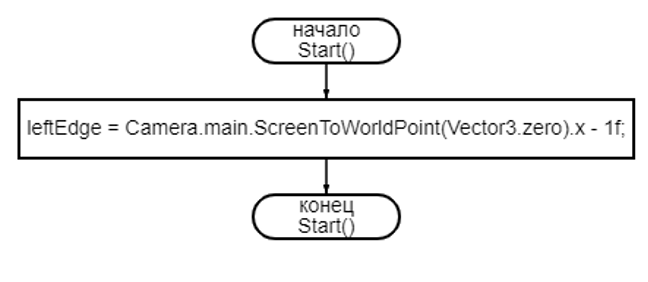
\includegraphics[scale=1.2]{p/PipeDOsnStart.png}}
\caption{Блок-схема для функции  Start() в классе PipeD.}
\end{figure}

\item Update()

\begin{figure}[H]
\center{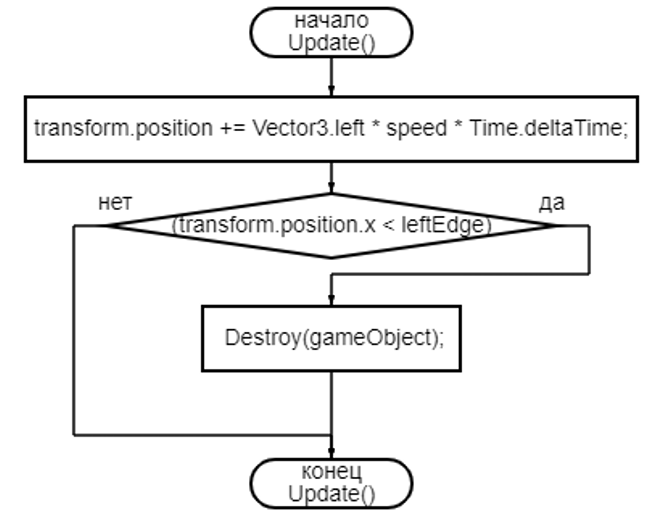
\includegraphics[scale=1.0]{p/PipeDOsnUpdate.png}}
\caption{Блок-схема для функции Update() в классе PipeD.}
\end{figure}

\end{enumerate}

\textbf{Подготовка и программирование интерфейса}

Создается объект «Canvas», в котором будут размещаться все объекты интерфейса. В нем дополнительно меняются параметры холста. UI Scale Mode = Scale With Screen Size. В Unity это определяет, как будет масштабироваться пользовательский интерфейс в зависимости от размера экрана. Когда установлен режим Scale With Screen Size, интерфейс автоматически масштабируется, чтобы соответствовать размеру экрана. 

Reference Resolution x = 1920, y = 1080. Так, когда используется режим Scale With Screen Size и указывается Reference Resolution, интерфейс будет автоматически масштабироваться, чтобы подходить к различным разрешениям экранов, сохраняя соотношение сторон.

«Canvas» содержит такие объекты как:

\begin{enumerate}
\item FlappyBird - компонент Image. В Source Image прикреплен спрайт под названием «FlappyBird». Данный компонент предназначен для создания красивой визуальной картинки на главном экране игры. Объект имеет расположение top - center с параметрами Pos X = 0, Pos Y = -240, Pos Z = 0, Widtg = 850, Height = 250, Rotation(0, 0, 0), Scale(1, 1, 1).
\item Ocho - компонент Text. В Text по умолчанию написан 0, используется шрифт Electronic Highway Sign для поддержания пиксельности игры, а также Font Size = 250. Horizontal и Vertical установлены на Overflow. Данный компонент предназначен для визуального отображения количества подсчитанных очков за трубы. Объект имеет расположение middle - center с параметрами Pos X = 0, Pos Y = 440, Pos Z = 0, Widtg = 0, Height = 0, Rotation(180, 0, 0), Scale(0.4, -0.4, 1).
\item GameOver - компонент Image. В Source Image прикреплен спрайт под названием «GameOver». Данный компонент предназначен для создания красивой визуальной картинки на экране завершенной игры. Объект имеет расположение middle - center с параметрами Pos X = 0, Pos Y = 420, Pos Z = 0, Widtg = 400, Height = 87.5, Rotation(0, 0, 0), Scale(1, 1, 1).
\item Button - компонент Button. В Source Image прикреплен спрайт под названием «PlayButton». Данный компонент предназначен для вызова запуска игры и обновления высоты труб. К кнопке прикреплен скрипт «Restart» и объект «Prefabs». Кнопка имеет расположение middle - center с параметрами Pos X = 0, Pos Y = -250, Pos Z = 0, Widtg = 200, Height = 87.5, Rotation(0, 0, 0), Scale(1, 1, 1). Также в On Click указан скрипт «GameManager» и прикреплен метод - «GameManager.Play» (скрипт «GameManager» будет расписан после описания всех объектов в «Canvas»).
\item Start - компонент Button. В Source Image прикреплен спрайт под названием «Start». Данный компонент предназначен для вызова старта игры. Кнопка имеет расположение middle - center с параметрами Pos X = 690, Pos Y = 400, Pos Z = 0, Widtg = 100, Height = 87, Rotation(0, 0, 0), Scale(1, 1, 1). Также в On Click указан скрипт «GameManager» и прикреплен метод - «GameManager.ContinueButtonPressed».
\item Pause - компонент Button. В Source Image прикреплен спрайт под названием «Pause». Данный компонент предназначен для вызова паузы игры. Кнопка имеет расположение middle - center с параметрами Pos X = 690, Pos Y = 400, Pos Z = 0, Widtg = 100, Height = 87, Rotation(0, 0, 0), Scale(1, 1, 1). Также в On Click указан скрипт «GameManager» и прикреплен метод - «GameManager.PauseButtonPressed».
\item Exit - компонент Button. В Source Image прикреплен спрайт под названием «Exit». Данный компонент предназначен для выхода из игры. Кнопка имеет расположение middle - center с параметрами Pos X = 800, Pos Y = 400, Pos Z = 0, Widtg = 100, Height = 87, Rotation(0, 0, 0), Scale(1, 1, 1). К кнопке прикреплен скрипт «Exit». Также в On Click указан скрипт «Exit» и прикреплен метод - «Exit.Quit»(скрипт «Exit» будет расписан после описания всех объектов в «Canvas»). 
\item AboutImage - компонент Image. В Source Image прикреплен спрайт под названием «AboutImage». Данный компонент предназначен для вывода информации о разработчике. Объект имеет расположение middle - center с параметрами Pos X = 0, Pos Y = 50, Pos Z = 0, Widtg = 1500, Height = 160, Rotation(0, 0, 0), Scale(1, 1, 1). 
\item HelpImage - компонент Image. В Source Image прикреплен спрайт под названием «H». Данный компонент предназначен для вывода информации об игре. Объект имеет расположение middle - center с параметрами Pos X = 0, Pos Y = 100, Pos Z = 0, Widtg = 1350, Height = 500, Rotation(0, 0, 0), Scale(1, 1, 1). 
\item HelpButton - компонент Button. В Source Image прикреплен спрайт под названием «Help». Данный компонент предназначен для вызова компонента «HelpImage». Кнопка имеет расположение middle - center с параметрами Pos X = 250, Pos Y = -250, Pos Z = 0, Widtg = 100, Height = 87.5, Rotation(0, 0, 0), Scale(1, 1, 1). Также в On Click указан скрипт «GameManager» и прикреплен метод - «GameManager.ToggleHelpImage».
\item AboutButton - компонент Button. В Source Image прикреплен спрайт под названием «About». Данный компонент предназначен для вызова компонента «AboutImage». Кнопка имеет расположение middle - center с параметрами Pos X = -250, Pos Y = -250, Pos Z = 0, Widtg = 100, Height = 87.5, Rotation(0, 0, 0), Scale(1, 1, 1). Также в On Click указан скрипт «GameManager» и прикреплен метод - «GameManager.ToggleAboutImage».
\item Panel - компонент Image. В Source Image прикреплен спрайт под названием «Panel». Данный компонент предназначен для оформления рекорда. Объект имеет расположение middle - center с параметрами Pos X = 0, Pos Y = 100, Pos Z = 0, Widtg = 800, Height = 500, Rotation(0, 0, 0), Scale(1, 1, 1). 
\item StartOcho - компонент Text. В Text по умолчанию написан 0, используется шрифт Electronic Highway Sign для поддержания пиксельности игры, а также Font Size = 200. Horizontal и Vertical установлены на Overflow. Данный компонент предназначен для визуального отображения количества подсчитанных очков за трубы. Объект имеет расположение middle - center с параметрами Pos X = 250, Pos Y = 245, Pos Z = 0, Widtg = 160, Height = 30, Rotation(0, 0, 0), Scale(0.5, -0.5, 1).
\item StartRecord - компонент Text. В Text по умолчанию написан 0, используется шрифт Electronic Highway Sign для поддержания пиксельности игры, а также Font Size = 200. Horizontal и Vertical установлены на Overflow. Данный компонент предназначен для визуального отображения количества максимально подсчитанных очков за трубы. Объект имеет расположение middle - center с параметрами Pos X = 20, Pos Y = 45, Pos Z = 0, Widtg = 160, Height = 30, Rotation(0, 0, 0), Scale(0.5, 0.5, 1).
\item StartOcho2 - компонент Image. В Source Image прикреплен спрайт под названием «StartOcho2». Данный компонент предназначен для указания начала очков. Объект имеет расположение middle - center с параметрами Pos X = -100, Pos Y = 200, Pos Z = 0, Widtg = 500, Height = 100, Rotation(0, 0, 0), Scale(1, 1, 1). 
\item StartRecord2 - компонент Image. В Source Image прикреплен спрайт под названием «StartRecord2». Данный компонент предназначен для указания рекордных очков. Объект имеет расположение middle - center с параметрами Pos X = -210, Pos Y = 0, Pos Z = 0, Widtg = 290, Height = 140, Rotation(0, 0, 0), Scale(1, 1, 1). 

\end{enumerate} 

Для управления интерфейсов был разработан скрипт «GameManager». Также создается дополнительно объект «GameManager», в котором к скрипту прикрепляются ссылки на объекты. 

В коде используются методы:

\begin{enumerate}
\item ToggleHelpAboutImage() - переключение видимости изображений в игровом интерфейсе. 
\item ToggleHelpAboutImage() - переключение видимости изображений в игровом интерфейсе для кнопки HelpButton.
\item ToggleAboutImage() - переключение видимости изображений в игровом интерфейсе для кнопки AboutButton.
\item Awake() - ставит игру сразу же на паузу пока пользователь не нажмет на кнопку запуска игры.
\item Start() - управление видимостью изображений на старте игры.
\item PauseButtonPressed() - вызов паузы для кнопки Pause и управление видимостью изображений.
\item ContinueButtonPressed() - вызов старта для кнопки Start и управление видимостью изображений.
\item Play() - устанавливает начальное значение очков, управляет видимостью объектов во время игры и активирует игровой объект player и трубы.
\item Pause() - останавливает игровой процесс и отключает игровой объект player.
\item GameOver() - используется для управления видимостью объектов в конце игры и для остановки игры и последующего ожидания, когда пользователь снова нажмет какую-либо кнопку.
\item IncreaseScore() - увеличивает счета игры при прохождении трубы и выводит счет на экран.
\item Update() - сравнивает каждый счет игры с рекордом и выводит максимальное кол-во очков как рекорд и выводит на экран.
\end{enumerate} 

Скрипт подробно расписан в приложении под заголовком «Управление интерфейсом».

\begin{figure}[H]
\center{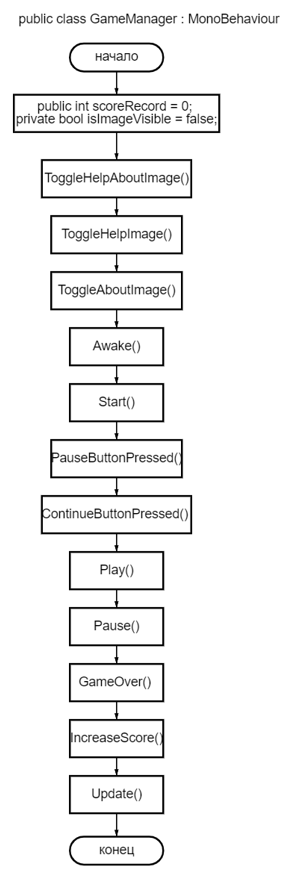
\includegraphics[scale=1.3]{p/GameManagerOsn.png}}
\caption{Блок-схема для класса GameManager.}
\end{figure}

Блок-схемы для функций в классе GameManager:
\begin{enumerate}
\item ToggleHelpAboutImage()

\begin{figure}[H]
\center{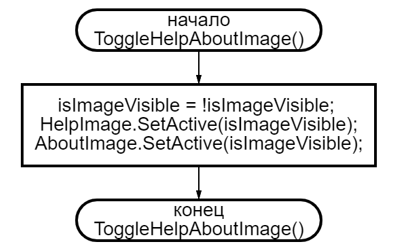
\includegraphics[scale=1.2]{p/GameManagerOsnToggeHelpAbout.png}}
\caption{Блок-схема для функции ToggleHelpAboutImage() в классе GameManager.}
\end{figure}

\item ToggleHelpImage()

\begin{figure}[H]
\center{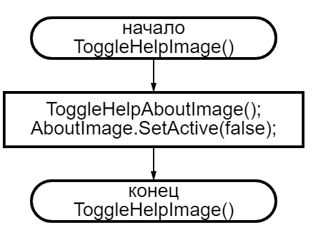
\includegraphics[scale=1.2]{p/GameManagerOsnToggeHelpImage.png}}
\caption{Блок-схема для функции ToggleHelpImage() в классе GameManager.}
\end{figure}

\item ToggleAboutImage()

\begin{figure}[H]
\center{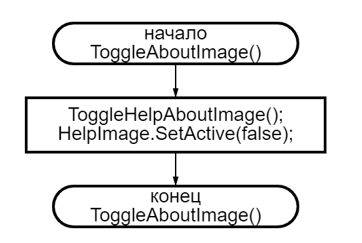
\includegraphics[scale=1.2]{p/GameManagerOsnToggeAboutImage.png}}
\caption{Блок-схема для функции ToggleAboutImage() в классе GameManager.}
\end{figure}

\item Awake()

\begin{figure}[H]
\center{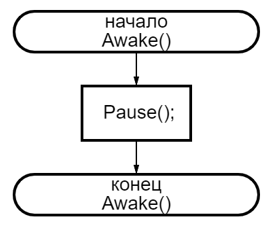
\includegraphics[scale=1.2]{p/GameManagerOsnAwake.png}}
\caption{Блок-схема для функции Awake() в классе GameManager.}
\end{figure}

\item Start()

\begin{figure}[H]
\center{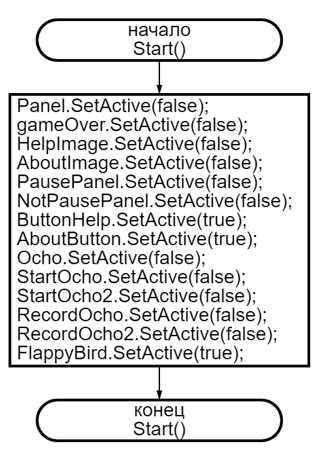
\includegraphics[scale=1.2]{p/GameManagerOsnStart.png}}
\caption{Блок-схема для функции Start() в классе GameManager.}
\end{figure}

\item PauseButtonPressed()

\begin{figure}[H]
\center{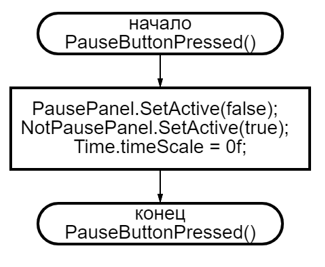
\includegraphics[scale=1.2]{p/GameManagerOsnPauseButton.png}}
\caption{Блок-схема для функции PauseButtonPressed() в классе GameManager.}
\end{figure}

\item ContinueButtonPressed()

\begin{figure}[H]
\center{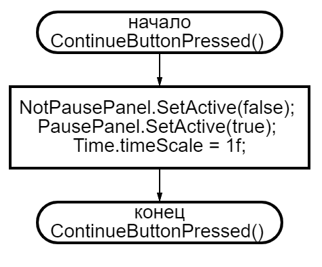
\includegraphics[scale=1.2]{p/GameManagerOsnCintinueButton.png}}
\caption{Блок-схема для функции ContinueButtonPressed() в классе GameManager.}
\end{figure}

\item Play()

\begin{figure}[H]
\center{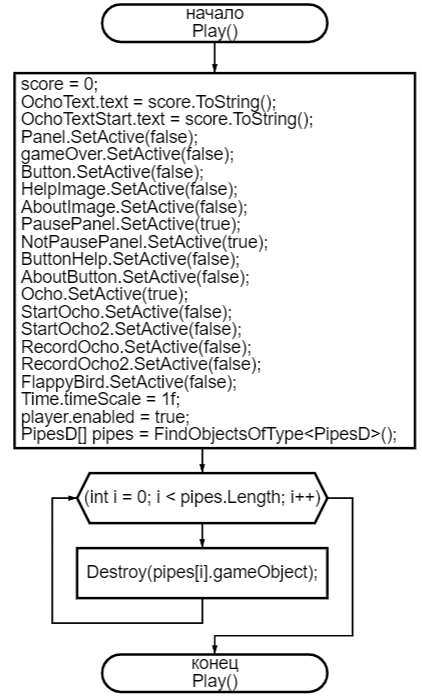
\includegraphics[scale=1.2]{p/GameManagerOsnPlay.png}}
\caption{Блок-схема для функции Play() в классе GameManager.}
\end{figure}

\item Pause()

\begin{figure}[H]
\center{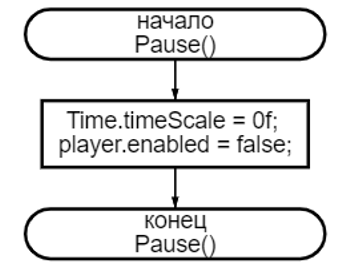
\includegraphics[scale=1.2]{p/GameManagerOsnPause.png}}
\caption{Блок-схема для функции Pause() в классе GameManager.}
\end{figure}

\item GameOver()

\begin{figure}[H]
\center{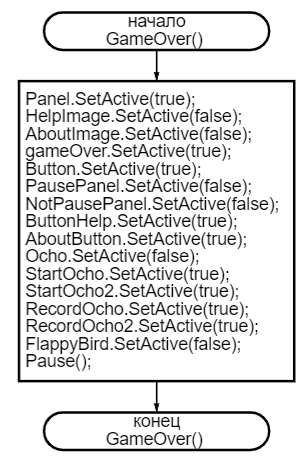
\includegraphics[scale=1.2]{p/GameManagerOsnGameOver.png}}
\caption{Блок-схема для функции GameOver() в классе GameManager.}
\end{figure}

\item IncreaseScore()

\begin{figure}[H]
\center{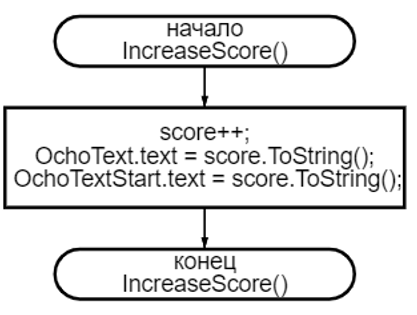
\includegraphics[scale=1.2]{p/GameManagerOsnIncreaseScore.png}}
\caption{Блок-схема для функции IncreaseScore() в классе GameManager.}
\end{figure}

\item Update()

\begin{figure}[H]
\center{\includegraphics[scale=1.2]{p/GameManagerOsnUpdate.png}}
\caption{Блок-схема для функции Update() в классе GameManager.}
\end{figure}

\end{enumerate}

Также дополнительно были разработаны скрипты «Exit» и «Restart».

«Exit» разработан для кнопки Exit, скрипт реализует выход из игры).

В коде используются методы:

\begin{enumerate}
\item Quit() - вызывает выход из приложения
\end{enumerate} 

Скрипт под названием «Exit» подробно расписан в приложении под заголовком «Код для кнопки Exit (выход из игры)».

\begin{figure}[H]
\center{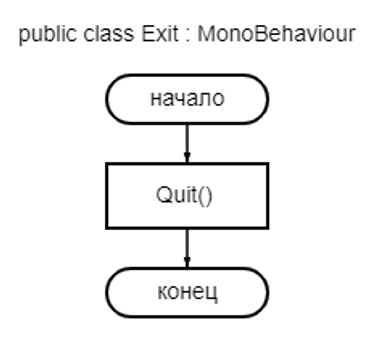
\includegraphics[scale=1.2]{p/ExitOsn.png}}
\caption{Блок-схема для класса Exit.}
\end{figure}

Блок-схемы для функций в классе Exit:
\begin{enumerate}
\item Quit()

\begin{figure}[H]
\center{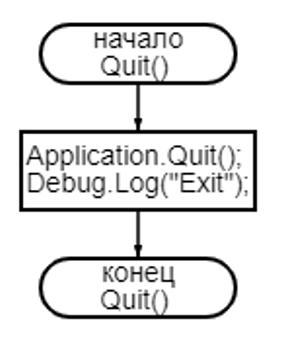
\includegraphics[scale=1.2]{p/ExitOsnQuit.png}}
\caption{Блок-схема для функции  Quit() в классе Exit.}
\end{figure}

\end{enumerate}

«Restart» для кнопки Button (скрипт реализует вызов метода ResetStartHeight(), что приводит к сбросу начальной высоты труб в скрипте Pipe) о которой ранее писалось. 

В коде используются методы:

\begin{enumerate}
\item Start() - вызывается при активации объекта Button. Получается ссылка на компонент и при нажатии кнопки следует вызов пользовательского метода ResetStartHeight().
\item ResetStartHeight() - вызывается при вызове метода ResetStartHeight() из скрипта Pipe, используя ссылку на объект pipe
\end{enumerate} 

Скрипт под названием «Restart» подробно расписан в приложении под заголовком «Код для кнопки Button (Cброс начальной высоты труб)».


\begin{figure}[H]
\center{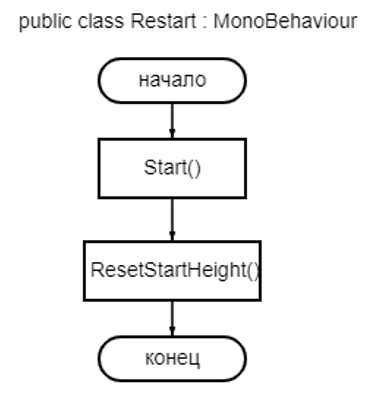
\includegraphics[scale=1.2]{p/RestartOsn.png}}
\caption{Блок-схема для класса Restart.}
\end{figure}

Блок-схемы для функций в классе Restart:
\begin{enumerate}
\item Start()

\begin{figure}[H]
\center{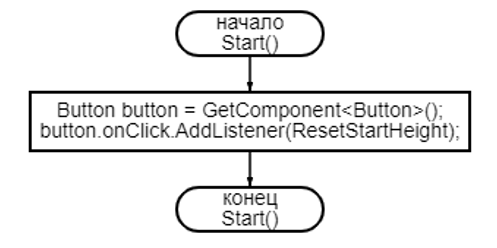
\includegraphics[scale=1.2]{p/RestartOsnStart.png}}
\caption{Блок-схема для функции  Start() в классе Restart.}
\end{figure}

\item ResetStartHeight()

\begin{figure}[H]
\center{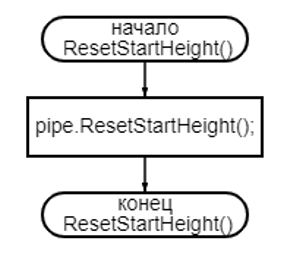
\includegraphics[scale=1.2]{p/RestartOsnRestartStart.png}}
\caption{Блок-схема для функции  ResetStartHeight() в классе Restart.}
\end{figure}

\end{enumerate}


\chapter*{Заключение}
\phantomsection\addcontentsline{toc}{chapter}{ЗАКЛЮЧЕНИЕ}

В целом, современные возможности создания игровых приложений позволяют разработчикам создавать увлекательные и качественные игры, которые могут быть доступны пользователям на разных платформах, не вызывая конфликтов и ограничений. Это открывает новые горизонты для игровой индустрии и предоставляет игрокам возможность наслаждаться играми, независимо от выбранной операционной системы или устройства.

Так, благодаря данной работе, было разработано игровое приложение «Flappy Bird» с помощью интегрированной среды разработки Unity и встроенного в него языка программирования С\#. С помощью упрощенного интерфейса разработки среды и использованию различных методов языка цель по созданию кроссплатформенной игры с графическим интерфейсом была достигнута.

\newpage
\phantomsection\addcontentsline{toc}{chapter}{СПИСОК ИСПОЛЬЗОВАННОЙ ЛИТЕРАТУРЫ}
\printbibliography[title={Список использованной литературы}]

\appendix
\newpage
\chapter*{\raggedleft\label{appendix1}Приложение}
\phantomsection\addcontentsline{toc}{chapter}{ПРИЛОЖЕНИЕ}
%\section*{\centering\label{code:appendix}Текст программы}

\begin{center}
\label{code:appendix}\textbf{Код для объекта «Player» (Птички)} 
\end{center}

using UnityEngine; 

public class Player : MonoBehaviour 

\{
    private SpriteRenderer spriteRenderer; //SpriteRenderer - отображает спрайты на экране

    public Sprite[] sprites; //Массив, содержит кол-во спрайтов для анимации

    private int spriteIndex; //Индекс спрайта

    private Vector3 direction; //Хранение инф. о направлении движения птички

    public float gravity = -9.8f; //Значение гравитации

    public float strenght = 5f; //Сила прыжка птички

    private void Awake() //Получение доступа к компоненту, отвечает за отображение спрайтов на экране и сохранение ее ссылки для взаимодействовий с др. методами

    \{

        spriteRenderer = GetComponent<SpriteRenderer>();

    \}

    private void Start() //Анимация спрайтов каждые 0.15 секунды

    \{

        InvokeRepeating(nameof(AnimateSprite), 0.15f, 0.15f);

    \}

    private void OnEnable() //Централизуем птичку при новой игре

    \{

        Vector3 position = transform.position;

        position.y = 0f; 

        transform.position = position;

        direction = Vector3.zero; 

    \}

    private void Update() //Вызывается каждый кадр, используется для обработки ввода пользователя и обновления состояния игрового объекта

    \{
       
        if (Input.GetKeyDown(KeyCode.Space) || Input.GetMouseButtonDown(0)) //Проверка нажатия пробела или л.к.м

        \{

            direction = Vector3.up * strenght; //Птичка будет совершать прыжок вверх с заданной силой

        \}

        direction.y += gravity * Time.deltaTime; //Позволяет птичке падать по гравитации, если не было прыжка

        transform.position += direction * Time.deltaTime; //Обновление позиции объекта, учитывая прошедшее время между кадрами
    \}
 
    private void AnimateSprite() //Анимация птички

    \{
        spriteIndex++; //Меняем индексы спрайтов
        
	//Если индекс превышает или = длине массива sprites, тоspriteIndex = 0 и анимация начинается с начала

        if (spriteIndex >= sprites.Length)

        \{

            spriteIndex = 0;

        \}

        spriteRenderer.sprite = sprites[spriteIndex]; // Вывод спрайта на экран

    \}

    private void OnTriggerEnter2D(Collider2D other)

    \{

        if (other.gameObject.tag == "Barrier") //Столкновение с объектом Barrier (верхней и нижней трубой)

        \{

            FindObjectOfType<GameManager>().GameOver(); //Поиска объекта с компонентом GameManager в сцене, завершение игры

        \}

        else if (other.gameObject.tag == "Ochos") //Столкновение с объектом Ochos (Часть промежутка трубы)

        \{

            FindObjectOfType<GameManager>().IncreaseScore(); //Поиска объекта с компонентом GameManager в сцене и увеличение счета очков

        \}

    \}

\}


\begin{center}
\label{code:appendix}\textbf{Код для объекта «Back» (Задний фон)} 
\end{center}

using UnityEngine;

public class Back : MonoBehaviour
\{
    private MeshRenderer meshRenderer;
    
    public float animationSpeed = 1f;

    private void Awake() //Получение доступа к компоненту, отвечает за отображение спрайтов на экране и сохранение ее ссылки для взаимодействовий с др. методами

    \{
    
        meshRenderer = GetComponent<MeshRenderer>();
        
    \}

    private void Update() // Вызывается каждый кадр, смещая текстуру (фон) 

    \{
    
        meshRenderer.material.mainTextureOffset += new Vector2(animationSpeed * Time.deltaTime, 0); //Значение по оси X равно произведению, y =  0
        
    \}
\}

\begin{center}
\label{code:appendix}\textbf{Код для объекта «Ground» (Передний фон)} 
\end{center}

using UnityEngine;

public class Ground : MonoBehaviour

\{
    private MeshRenderer meshRenderer;
    
    public float animationSpeed = 0.75f;

    private void Awake() //Получение доступа к компоненту, отвечает за отображение спрайтов на экране и сохранение ее ссылки для взаимодействовий с др. методами

    \{
    
        meshRenderer = GetComponent<MeshRenderer>();
        
    \}

    private void Update() // Вызывается каждый кадр, смещая текстуру (фон) 

    \{
        
        meshRenderer.material.mainTextureOffset += new Vector2(animationSpeed * Time.deltaTime, 0); //Значение по оси X равно произведению, y =  0
        
    \}
\}

\begin{center}
\label{code:appendix}\textbf{«Код для объекта Prefabs (Спавн труб)»} 
\end{center}

using UnityEngine;

public class Pipe : MonoBehaviour

\{

    public GameObject prefab; //Хранение изготовленного префаба

    public float spawnRate = 1.0f; //Частота спавна новых труб = 1 секунде

    public float minHeight = -3.0f; //Минимальная высота спавна трубы
    
    public float maxHeight = 3.0f; //Максимальная высота спавна трубы

    public float startminHeight = 0.0f; //Минимальная начальная высота спавна трубы
    
    public float startmaxHeight = 0.0f; //Максимальная начальная высота спавна трубы

    private void OnEnable() //Вызов метода каждую секунду для создания труб 
    
    \{
        
        InvokeRepeating(nameof(Spawn), spawnRate, spawnRate);
    
    \}

    private void Spawn() //Создание новой трубы на основе префаба с генерацией случайной высоты в изменяющемся диапазоне
    
    \{
    
        float randomHeight = Random.Range(startminHeight, startmaxHeight); // Генерация случайной высоты в диапазоне

        Vector3 spawnPosition = transform.position + new Vector3(0, randomHeight, 0); // Позиция созданной трубы с учетом случайной высоты

        GameObject newPipe = Instantiate(prefab, spawnPosition, Quaternion.identity); // Создание новой трубы на основе префаба

        if (startminHeight> minHeight \&\& startmaxHeight < maxHeight) //Увеличение диапазона

        \{
            startminHeight += -0.1f; //Минимальная начальная высота спавна трубы
            startmaxHeight += 0.1f; //Максимальная начальная высота спавна трубы

        \}
        
    \}

    public void ResetStartHeight() //Сброс начальной высоты спавна труб, чтобы на старте трубы снова спавнились с простого положения
    
    \{
    
        startminHeight = 0.0f;
        startmaxHeight = 0.0f;
        
    \}

\}


\begin{center}
\label{code:appendix}\textbf{«Код для префаба Pipes (Движение труб)»} 
\end{center}

using UnityEngine;

public class Pipes : MonoBehaviour

\{
    public float speed = 4.0f; //Скорость движения объекта

    private float leftEdge; //Хранения координаты левого края экрана

    private void Start() //Получение координаты x левого главного экрана сцены и вычет промежутка, чтобы трубы исчезали чуть позже 
    
    \{
    
        leftEdge = Camera.main.ScreenToWorldPoint(Vector3.zero).x - 1f;
        
    \}

    private void Update() //Вызывается для перемещения труб влево, +проверяется, достигла ли труба левого края экрана для дальнейшего уничтожения

    \{
    
        transform.position += Vector3.left * speed * Time.deltaTime; //Перемещает трубы влево на установленный 

        if (transform.position.x < leftEdge) //Проверка на достижение трубой левого края
        
        \{
        
            Destroy(gameObject); //Если достигла - уничтожается
            
        \}
        
    \}

\}


\begin{center}
\label{code:appendix}\textbf{«Код для кнопки Exit (выход из игры)»} 
\end{center} 

using UnityEngine;

public class Exit : MonoBehaviour

\{
    public void Quit() //Вызывается для выхода из приложения
    
    \{
    
        Application.Quit(); //Завершает выполнение приложения, когда метод вызывается
        
        Debug.Log("Exit"); //Вывод сообщения "Exit" в консоль Unity
        
    \}
    
\}


\begin{center}
\label{code:appendix}\textbf{«Код для кнопки Button (Cброс начальной высоты труб)»} 
\end{center} 

using UnityEngine;

using UnityEngine.UI;

public class Restart : MonoBehaviour

\{

    public Pipe pipe; // Ссылка на скрипт Pipe

    private void Start()
    
    \{
        Button button = GetComponent<Button>(); //Ссылка на кнопку
        
        button.onClick.AddListener(ResetStartHeight); //При нажатии на эту кнопку будет вызываться метод ResetStartHeight()
    
    \}

    private void ResetStartHeight() //Вызов метода ResetStartHeight() из скрипта Pipe, используя ссылку на объект pipe
    
    \{
        
        pipe.ResetStartHeight();
    
    \}

\}

\begin{center}
\label{code:appendix}\textbf{«Управление интерфейсом»} 
\end{center} 

using UnityEngine;

using UnityEngine.UI;

public class GameManager : MonoBehaviour

\{
    public Player player; //Ссылка на скрипт Player

    public Text OchoText; //Ссылка на компонент Text с отображением очков

    public Text OchoTextStart; //Ссылка на компонент Text с отображением очков

    public Text OchoTextRecord; //Ссылка на компонент Text с отображением рекордных очков

    public GameObject Ocho; //Ссылка на объект в игровом интерфейсе 

    public GameObject StartOcho;

    public GameObject StartOcho2;

    public GameObject RecordOcho;

    public GameObject RecordOcho2;

    public GameObject Panel;

    public GameObject gameOver;

    public GameObject Button;

    public GameObject ButtonHelp;

    public GameObject AboutButton;

    public GameObject PausePanel;

    public GameObject NotPausePanel;

    public GameObject FlappyBird;

    public int score; //Счетчик очков

    public int scoreRecord = 0; //Счетчик рекордных очков

    
    [SerializeField] GameObject HelpImage; //Ссылка на отображение изображения
    
    [SerializeField] GameObject AboutImage; //Ссылка на отображение изображения

    private bool isImageVisible = false; //Отслеживание видимости изображений

    public void ToggleHelpAboutImage()
    
    \{
        isImageVisible = !isImageVisible; //Переключения флага между true и false, чтобы контролировать видимость изображений в методах
        
        HelpImage.SetActive(isImageVisible); //Объект скрыт на сцене
        
        AboutImage.SetActive(isImageVisible); //Объект скрыт на сцене

    \}

    public void ToggleHelpImage() //Вызов для кнопки HelpButton
    
    \{
    
        ToggleHelpAboutImage(); //Вызов метода для переключения флагов
        
        AboutImage.SetActive(false); //Объект скрыт на сцене
        
    \}

    public void ToggleAboutImage() //Вызов для кнопки AboutButton
    
    \{
    
        ToggleHelpAboutImage(); //Вызов метода для переключения флагов
        
        HelpImage.SetActive(false); //Объект скрыт на сцене
        
    \}
    

    public void Awake() //Пауза, пока не нажмется кнопка старта
    
    \{
    
        Pause();
        
    \}

    public void Start() //Вызывается чтобы убрать/показать объекты в начале запуска игры 
    
    \{
        Panel.SetActive(false);
        
        gameOver.SetActive(false);
        
        HelpImage.SetActive(false);
        
        AboutImage.SetActive(false);

        PausePanel.SetActive(false);
        
        NotPausePanel.SetActive(false);
        
        ButtonHelp.SetActive(true);
        
        AboutButton.SetActive(true);

        Ocho.SetActive(false);
        
        StartOcho.SetActive(false);
        
        StartOcho2.SetActive(false);
        
        RecordOcho.SetActive(false);
        
        RecordOcho2.SetActive(false);
        
        FlappyBird.SetActive(true);


    \}

    
    public void PauseButtonPressed() //Вызов паузы для кнопки Pause
    
    \{
    
        PausePanel.SetActive(false); 
        
        NotPausePanel.SetActive(true);

        Time.timeScale = 0f; //ставим скорость проигрывания на 0
    
    \}

    public void ContinueButtonPressed() //Вызов старта для кнопки Start
    
    \{
    
        NotPausePanel.SetActive(false);
        
        PausePanel.SetActive(true);
        
        Time.timeScale = 1f; //ставим скорость проигрывания на 1 
        
    \}
    

    public void Play() //Вызывается чтобы убрать/показать объекты во время игры 
    
    \{
        score = 0;

        OchoText.text = score.ToString(); //Вывод очков на экран с помощью свойства text

        OchoTextStart.text = score.ToString(); //Вывод очков на экран с помощью свойства text

        Panel.SetActive(false);
        
        gameOver.SetActive(false);
        
        Button.SetActive(false);
        
        HelpImage.SetActive(false);
        
        AboutImage.SetActive(false);
        
        PausePanel.SetActive(true);
        
        NotPausePanel.SetActive(true);
        
        ButtonHelp.SetActive(false);
        
        AboutButton.SetActive(false);
        
        Ocho.SetActive(true);
        
        StartOcho.SetActive(false);
        
        StartOcho2.SetActive(false);
        
        RecordOcho.SetActive(false);
        
        RecordOcho2.SetActive(false);
        
        FlappyBird.SetActive(false);

        Time.timeScale = 1f; //Снятие игры с паузы
        
        player.enabled = true; //Включение объекта Player

        PipesD[] pipes = FindObjectsOfType<PipesD>(); //Создание массива типа PipesD и выполнение поиска всех объектов на сцене, которые являются экземплярами класса PipesD 

        for (int i = 0; i < pipes.Length; i++) //Перебор элементов массива pipes и уничтожение каждого объект, на который указывает элемент pipes[i]
        
        \{
        
            
            Destroy(pipes[i].gameObject);
        
        \}
    \}

    public void Pause() //Прописываем параметры паузы
    
    \{
    
        Time.timeScale = 0f; //ставим скорость проигрывания на 0
        
        player.enabled = false; //Выключение объекта Player
        
    \}

    public void GameOver() //Вызывается чтобы убрать/показать объекты в конце игры
    
    \{
    
        Panel.SetActive(true);
        
        HelpImage.SetActive(false);
        
        AboutImage.SetActive(false);
        
        gameOver.SetActive(true);
        
        Button.SetActive(true);

        PausePanel.SetActive(false);
        
        NotPausePanel.SetActive(false);

        ButtonHelp.SetActive(true);
        
        AboutButton.SetActive(true);

        Ocho.SetActive(false);
        
        StartOcho.SetActive(true);
        
        StartOcho2.SetActive(true);
        
        RecordOcho.SetActive(true);
        
        RecordOcho2.SetActive(true);
        
        FlappyBird.SetActive(false);

        Pause(); //Ждем когда пользователь опять нажмет какую-то кнопку
        
    \}

    public void IncreaseScore() //Набор очков +1, если птичка попадает в область между труб
    
    \{
    
        score++;
        
        OchoText.text = score.ToString(); //Вывод очков на экран с помощью свойства text
        
        OchoTextStart.text = score.ToString(); //Вывод очков на экран с помощью свойства text
        
    \}


    public void Update() //Пересчитываем каждый раз количество очков и находим рекордное
    
    \{

        if (scoreRecord <= score)
        
        \{
        
            scoreRecord = score;
            
            OchoTextRecord.text = score.ToString(); //Вывод рекорда на экран с помощью свойства text

        \};
        
    \}

\}


\end{document}
